% article_FR.tex — one-page presentation of WAC for a DFIR magazine, French
% edition. The English edition is article_EN.tex, in this folder: both are
% maintained together, paragraph for paragraph.
%
% Build (LuaLaTeX, as the editor's recipe; build artefacts removed after):
%     ../build-docs.sh article_FR.tex
%
% Every figure comes from the comparison, validation and harmlessness files
% (doc/comparison, doc/validation, doc/harmlessness), measured on 9 October 2026
% on version 2.0.0. Backlog B-018.

\documentclass[10pt,a4paper,twocolumn]{article}
\usepackage[french]{babel}
\usepackage{fontspec}
\setmainfont{Noto Sans}
\setmonofont{DejaVu Sans Mono}[Scale=0.84]
\usepackage[top=13mm,bottom=13mm,left=14mm,right=14mm,columnsep=7mm]{geometry}
\usepackage{xcolor}
\usepackage{titlesec}
\usepackage{enumitem}
\usepackage{array}
\usepackage{graphicx}
\usepackage{caption}
\captionsetup{font={small,color=gris},skip=2pt}
\usepackage[hidelinks]{hyperref}
\definecolor{marine}{HTML}{0A1A33}
\definecolor{bleu}{HTML}{2F6DB5}
\definecolor{gris}{HTML}{5B6573}
\pagestyle{empty}
\setlength{\parindent}{0pt}
\setlength{\parskip}{0.35em}
\titleformat{\section}{\color{marine}\normalsize\bfseries}{}{0em}{}
\titlespacing*{\section}{0pt}{0.7em}{0.2em}
\setlist{nosep,leftmargin=1.1em}
\newcommand{\wac}{\textsc{wac}}
\newcommand{\fichier}[1]{\texttt{#1}}
\hypersetup{pdftitle={WAC — collecter Windows sans y laisser de trace}}

\begin{document}

\twocolumn[{%
  {\color{marine}\LARGE\bfseries WAC : collecter Windows sans y laisser de trace}\par
  \vspace{0.3em}
  {\color{gris}Centre d'Excellence Cyberdéfense Aérospatiale (CEC), École de l'air et de l'espace}\par
  \vspace{0.6em}
  {\itshape Une collecte se fait sur une machine qui est aussi une preuve. L'outil
  qui la prélève doit tout prendre, ne rien y écrire, et pouvoir le démontrer.
  \wac{} (Windows Artefacts Collector), logiciel libre écrit en C++, prélève
  69 artefacts d'un poste Windows en lecture brute, les convertit en JSON sur
  le poste d'analyse, scelle et journalise chacune de ses opérations. Ses
  résultats ont été confrontés, valeur par valeur, à ceux de KAPE et des
  outils d'Eric Zimmerman.}\par
  \vspace{0.9em}
}]

\section{Ce qui est prélevé}
Un seul exécutable autonome, lancé depuis une clé, lit les volumes NTFS en
brut : \fichier{\$MFT} et index des répertoires, sans ouvrir un fichier. Les
fichiers verrouillés (ruches, journaux) sont lus comme les autres, et aucune
date d'accès ne change. 69 artefacts : ruches système et de chaque profil (SAM
en entier, BAM, UserAssist, ShimCache, Amcache, shellbags, USB),
\fichier{\$MFT}, \fichier{\$UsnJrnl}, \fichier{\$LogFile}, journaux
d'événements avec les ressources qui en donnent le texte, Prefetch, raccourcis,
jump lists, SRUM, corbeille, tâches planifiées, WMI, persistance, Defender,
navigateurs (historique, téléchargements, sessions et onglets fermés),
courrier, clés DPAPI, volumes FAT et exFAT des clés USB. Les exécutables de la
machine sont lus et leur signature Authenticode vérifiée en mémoire : un
binaire Microsoft authentique n'est consigné que par ses empreintes, tout
autre est copié. Face à KAPE (\fichier{KapeTriage}), \wac{} prend tout ce que
KAPE prend --- hormis 5 \fichier{desktop.ini} --- et 790 fichiers de plus, en
41~s contre 44.

\section{Une procédure respectée}
\wac{} \emph{collecte} sur la machine examinée ou \emph{convertit} sur le poste
d'analyse, jamais les deux. Chaque pièce entre dans une \textbf{consigne}
scellée : son manifeste donne, pour chacune, MD5, SHA-1 et SHA-256, les huit
dates NTFS de l'original (\fichier{\$STANDARD\_INFORMATION} et
\fichier{\$FILE\_NAME}), son entrée MFT et la méthode de lecture ; l'empreinte
du manifeste le scelle. Après la copie initiale, la consigne n'est plus ni lue
ni écrite : la conversion vérifie d'abord le sceau et chaque empreinte, refuse
une pièce retouchée, puis travaille sur une copie de travail, où sont rejoués
les journaux des ruches et des bases ESE. Chaque opération est inscrite dans
le \textbf{journal d'investigation} (\fichier{investigation.json}) : instant,
cible, résultat, trace qu'elle est censée laisser, et durée de chaque étape.
Deux scripts livrés revérifient une consigne sans \wac{}.

\section{Du JSON, pas du CSV}
Un fichier par artefact, des valeurs typées (nombres, booléens, listes
imbriquées), chaque date au 100\,ns en UTC et en heure locale du suspect, avec
le décalage en vigueur \emph{à cette date}. Un champ sans valeur n'est pas
émis : ni zéro ni date 1601 qui se liraient comme une donnée. Le texte de
chaque événement est rendu comme l'affiche Windows. Le résultat se charge tel
quel dans un outil d'analyse.

\section{Aucune trace, mesurée}
Sur un clone figé de la machine de test, chaque outil est lancé depuis une clé,
sous Sysmon, le journal des modifications NTFS borné avant et après. \wac{}
n'écrit \textbf{aucun fichier} sur C:, \textbf{aucune valeur de registre},
aucun événement dans les journaux de Windows ; il ne lance aucun processus et
n'émet rien sur le réseau. Restent l'entrée Amcache et l'entrée ShimCache que
Windows crée pour tout programme, et ce qu'une surveillance enregistre de son
exécution (Sysmon : le processus, deux lectures brutes de volume). Dans les
mêmes conditions, KAPE écrit dans la ruche de l'utilisateur, et ses modules
28 fichiers sur C:. Le script de compilation refuse un \fichier{WAC.exe} qui
importerait une fonction capable de lancer un processus.

\section{Des tests qui savent échouer}
Un cycle autonome, dans une machine virtuelle Windows~11, pose des témoins de
valeur connue (fichiers, registre, navigateurs, courrier, un chemin de
261~caractères), collecte, convertit, et passe 494 contrôles. Chacun confronte
\wac{} à une source indépendante : Windows lui-même (\fichier{Get-WinEvent},
\fichier{Get-FileHash}, registre), \fichier{dissect.esedb}, le SQLite et le
\fichier{lz4} de Python. Une seconde conversion doit donner les mêmes JSON,
octet pour octet. Face aux onze outils d'Eric Zimmerman, sur les mêmes pièces,
chaque écart a été tranché par une telle source : les valeurs de \wac{} sont
les mêmes, ou plus justes (RECmd ramène des ruches à un état ancien,
AmcacheParser invente 3\,450 valeurs, EvtxECmd se trompe sur dix).

\section{En chiffres}
\begin{tabular}{@{}>{\raggedright\arraybackslash}p{0.8\columnwidth}@{\hspace{0.5em}}r@{}}
Artefacts prélevés & 69 \\
Collecte sans les exécutables (KAPE : 44~s) & 41~s \\
Conversion complète, consigne vérifiée & 80~s \\
Fichiers écrits sur C: par \wac{} & 0 \\
Contrôles du cycle de test & 494 \\
Outils de référence confrontés & 12 \\
\end{tabular}

\section{Disponibilité}
Version 2.0.0, Windows~10 et 11 (x64), licence GPL~3.0 :
\url{https://github.com/dev-cec/WAC}. Manuels, dossiers de validation,
d'innocuité et de comparaison en français et en anglais.


\vfill
\begin{center}
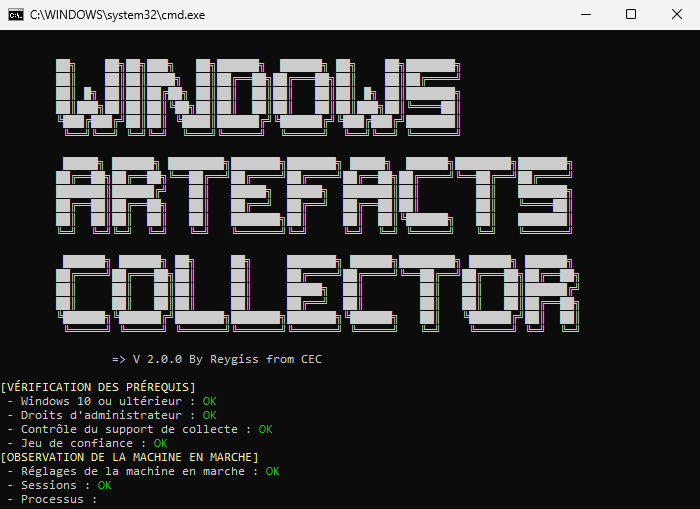
\includegraphics[width=\columnwidth,height=46mm,keepaspectratio]{../images/wac-running_FR.png}
\captionof*{figure}{\wac{} en cours de collecte.}
\end{center}

\end{document}
